\chapter{Implementation and Results}
\section{Groth16 proof and verification}
Let us use an example to illustrate the underlying mathematical methods that are applied in zk-SNARK algorithms. 

Say we want to prove we know a secret x so that

\[x^3 + x + 5 = 35\]

In this case, our secret is x = 3.
In practice, we would use Hiding and Modular Arithmetic instead of real numbers and calculations since these are easy to forge and find solutions to, which will make the proof useless. For R1CS and QAP we will proceed with real numbers examples to show the underlying mechanisms. The next two sub chapters will demonstrate how any computation that needs to be proven can be converted into polynomial format.

\subsubsection{Arriving at a R1CS}

A rank-1 constraint system is a mathematical format to help us reduce our problem into a less complex problem. First, we flatten the equation by writing a short program that would break down the different steps to solve the equation.

\begin{enumerate}
    \item \(sum1 = x * x\)
    \item \(y = sum1 * x\)
    \item \(sum2 = y + x\)
    \item \(out = sum2 + 5\)
\end{enumerate}

As shown above, we arrive at 4 gates with the solution variables
\[x = 3, y = 27, sum1 = 9, sum2 = 30, out = 35.\]

From this, we can construct the solution vector s, which has to start with a dummy variable of value 1, which we call \textit{one}.
Now, the solution vector s is
\begin{align}
    \Vec{s} &= \begin{pmatrix}
     one \\ x \\ out \\ sum1 \\ y \\ sum2
\end{pmatrix}
\end{align}
Each gate will be represented so that
\begin{align}
     \Vec{s}\cdot\Vec{a} * \Vec{s}\cdot\Vec{b} - \Vec{s}\cdot\Vec{c} = 0
\end{align}

Let us go through every gate and assign the values for a, b and c.
For the first gate \(sum1 = x*x\), the values of a, b and c are assigned as follows:
\begin{align*}
    a &=\begin{bmatrix}
        0 & 1 & 0 & 0 & 0 & 0
    \end{bmatrix}
\end{align*}
\begin{align*}
    b&=\begin{bmatrix}
        0 & 1 & 0 & 0 & 0 & 0 
    \end{bmatrix}
\end{align*}
\begin{align*}
    c&=\begin{bmatrix}
        0 & 0 & 0 & 1 & 0 & 0
    \end{bmatrix}
\end{align*}

This is correct, because the dot product of s and a, multiplied by the dot product of a and b, subtracted by the dot product of s and c is 0 (see (2)).

This procedure is applied for every gate. Let us show more complex gates to underline the calculation. For example, the third gate and the fourth gate. The third gate \(sum2=y+x\) could be approached like the first gate, by setting the variables in the equation to 1. However, this would not fulfill the equation shown in (2). Therefore, the correct values for a, b, and c are
\begin{align*}
    a &=\begin{bmatrix}
        0 & 1 & 0 & 0 & 0 & 0
    \end{bmatrix}
\end{align*}
\begin{align*}
    b&=\begin{bmatrix}
        1 & 0 & 0 & 0 & 0 & 0 
    \end{bmatrix}
\end{align*}
\begin{align*}
    c&=\begin{bmatrix}
        0 & 0 & 0 & 0 & 0 & 1
    \end{bmatrix}
\end{align*}

Here, we make use of the dummy vector \textit{one}, so that we can arrive at 
\[30 * 1 - 30 = 0.\]

The fourth gate \(out=sum2+5\) also has to be approached by holding true to the dot product equation in (2). We have to make use of the dummy vector once again. Setting the values of one, sum2 and out to 1 will give us the following incorrect solution:
\begin{align*}
     \Vec{s}\cdot\Vec{a} * \Vec{s}\cdot\Vec{b} - \Vec{s}\cdot\Vec{c} \neq 0.
\end{align*}
The calculation shows \(30 * 1 - 35 \neq 0\), which means we need to add 5, so that the dot product of vector s and a adds up to 35. Therefore, the values of a, b and c for the fourth gate are as follows:
\begin{align*}
    a &=\begin{bmatrix}
        5 & 0 & 0 & 0 & 0 & 1
    \end{bmatrix}
\end{align*}
\begin{align*}
    b&=\begin{bmatrix}
        1 & 0 & 0 & 0 & 0 & 0 
    \end{bmatrix}
\end{align*}
\begin{align*}
    c&=\begin{bmatrix}
        0 & 0 & 1 & 0 & 0 & 0
    \end{bmatrix}
\end{align*}

By combining our results as follows, we can set up the corresponding R1CS:

\begin{align}
A&=\begin{pmatrix}
    0 & 1 & 0 & 0 & 0 & 0 \\
    0 & 0 & 0 & 1 & 0 & 0 \\
    0 & 1 & 0 & 0 & 1 & 0 \\
    5 & 0 & 0 & 0 & 0 & 1
\end{pmatrix}
\end{align}
\begin{align*}
B&=\begin{pmatrix}
    0 & 1 & 0 & 0 & 0 & 0 \\
    0 & 1 & 0 & 0 & 0 & 0 \\
    1 & 1 & 0 & 0 & 0 & 0 \\
    1 & 0 & 0 & 0 & 0 & 0
\end{pmatrix}
\end{align*}
\begin{align*}
C&=\begin{pmatrix}
    0 & 0 & 0 & 1 & 0 & 0 \\
    0 & 0 & 0 & 0 & 1 & 0 \\
    0 & 0 & 0 & 0 & 0 & 0 \\
    0 & 0 & 1 & 0 & 0 & 0
\end{pmatrix}
\end{align*}

\subsubsection{From a R1CS to QAP}

The R1CS shows three matrices A, B, C representing the four gates each of length six. It is transformed into a Quadratic Arithmetic Program (QAP) by expressing polynomials as sums of Lagrange Interpolation. This results in three sets of polynomials A, B and C, each consisting of six polynomials of degree three. In the following, we will summarize the reason of setting up a QAP instead of continuing with the R1CS. From now on, A, B, C will be referred to as matrices with polynomial coefficients as values instead of the numbers seen above. Lagrange Interpolation allows us to come up with polynomial coefficients, which represent each gate, when evaluated at an x in the range of number of constraints (gates). With x = 1, the Lagrange Interpolation can be explained quite well, because it means that we can just add up the coefficients of the polynomials in A, B and C. Each set of polynomial is built so that evaluated at an x, whereby x has to be in the range of the number of gates (constraints), will deliver the specific value of x and 0 for the other values in that specific range.

The QAP for our example is shown as follows:

\begin{align*}
    A \\
    \begin{bmatrix}
        -5.0 & 9.166 & -5.0 & 0.833 \\
        8.0 & -11.33 & 5.0 & -0.666 \\
        0.0 & 0.0 & 0.0 & 0.0 \\
        -6.0 & 0.5 & -4.0 & 0.5 \\
        4.0 & -7.0 & 3.5 & -0.5 \\
        -1.0 & 1.833 & -1.0 & 0.166
    \end{bmatrix} \\
\end{align*}
\begin{align*}
        B \\
    \begin{bmatrix}
        3.0 & -5.166 & 2.5 & -0.333 \\
        -2.0 & 5.166 & -2.5 & 0.333 \\
        0.0 & 0.0 & 0.0 & 0.0 \\
        0.0 & 0.0 & 0.0 & 0.0 \\
        0.0 & 0.0 & 0.0 & 0.0 \\
        0.0 & 0.0 & 0.0 & 0.0
    \end{bmatrix}
\end{align*}
\begin{align*}
        C \\
    \begin{bmatrix}
        0.0 & 0.0 & 0.0 & 0.0 \\
        0.0 & 0.0 & 0.0 & 0.0 \\
        -1.0 & 1.833 & -1.0 & 0.166 \\
        4.0 & -4.833 & 1.5 & -0.166 \\
        -6.0 & 9.5 & -4.0 & 0.5 \\
        4.0 & -7.0 & 3.5 & -0.5
    \end{bmatrix}
\end{align*}
The corresponding values in A, B and C represent polynomial coefficients and shall be read from right to left, e.g. \(A1(X) = 0.833x^3 - 5x^2 + 9.166x -5\).

For example, evaluating A, B and C at x = 1 means to adding up the coefficients of the first polynomial of A, which will result in a value. Then, the next polynomial in A etc. It will result in a vector of length six and will be correct if the values match vector a from the first gate in our R1CS.
However, it would be cumbersome to evaluate each constraint of the R1CS individually. This is why we can make use of the QAP to check whether the dot product equation of the polynomials will hold:
\begin{align}
    A\cdot \Vec{s} * B\cdot \Vec{s} - C\cdot \Vec{s} = H(X) * Z(X)
\end{align}
Interestingly, the left side of the equation is our target polynomial T(X), which we want to proof. Also, \(A \cdot \Vec{s} = A(X), B \cdot \Vec{s} = B(X),  C \cdot \Vec{s} = C(X).\) 
Therefore, \(T(X) = A(X) * B(X) - C(X)\), which should be already familiar by revisiting (2), but this time the inputs are polynomials.
Now, let's have a look at the right side of the equation in (4). Z(X) is known if we know the number if constraints. In this case, we have four gates, so we arrive at
\begin{align}
    Z(X) = (x-1)(x-2)(x-3)(x-4)
\end{align}
H(X) is the hiding of our initial minimal example, those input we don't want to share, but proof we know the solution to. What role Hiding plays will be explained later. Now, we want to still finish looking at the equation in (4). In essence, we want to proof we know a polynomial and its solution, so that
\begin{align}
    T(X) / Z(X) = H(X)
\end{align}
Ultimately, in our example H(X) is also a polynomial. We know the QAP is correct, if H(X) is a polynomial without remainder. In this example, the resulting
\[H(X) = -0.44x^3 + 17.055x^2 - 3.666x.\]

Practically, the coefficients of each polynomial in A, B and C are publicly known. The same can be said for Z(X) through knowing the number of constraints (in this example we have four constraints. The prover can use the circuit to create vector s, calculate A(X), B(X) and C(X), as well as T(X). Subsequently, the prover can calculate the coefficients of H(X) by dividing T(X) / Z(X). However, there is no zero-knowledge yet, since the prover has to prove knowledge of vector s and H(X) without revealing it.
\newpage

\subsubsection{Hiding}
As touched upon earlier, there are information made publicly known. Zk-SNARKs are dependent on a trusted set-up releasing these parameters. The goal is to prove knowledge of the polynomial H(X) with all its coefficients without disclosing any of this information. Therefore, the trusted set-up also provides a random secret point P. Note, that P is hashed, calculated once and deleted from memory. Depending on the number of constraints, a certain amount of P values are needed. In our example, we have four constraints, which needs \(P = {1, P, P^2, P^3}\), whereby the value of \(P^3\) corresponds to the value of \(x^3\) when the polynomials are evaluated. The following values of P are provided

\begin{align}
    hh(1), hh(P), hh(P^2), ..., hh(P^\textsuperscript{(no. of constraints - 1)})
\end{align}

The trusted set-up makes these values publicly available in the CRS (Common Reference String).

With our previous knowledge, we know that the prove will be
\begin{align}
    \frac{hh[A(P)] * hh[B(P)] - hh[C(P)])}{hh[Z(P)]} = hh[H(P)]
\end{align}

The hidings of our polynomials are numbers, that currently can just be forged. The following will show how it can be proven that these numbers are hidings of the polynomials A(X), B(X) and C(X) in P, which is not known to anybody. Furthermore, we need to prove that in order to arrive at A(X), B(X) and C(X), the same solution vector s was used (see (4)). 

In order to approach the first problem, proving that the hidings of A(X),  B(X) and C(X) were actually calculated in P, we need to "extend" P by the same number, namely \(u\). The CRS consists also of \(hh(u*P), hh(u*P^2), hh(u*P^3)\), etc., i.e., it consists of two sets of hidings. We know that A(X) is a linear combination of the values of vector s inserted into the polynomials A1, A2, A3, etc. of A. B calculating \(hh[A(P)]\) and \(hh[A(u*P)]\) and looking if \(hh[A(P)] = u * hh[A(u*P]\) holds true, shows that the hiding of A(X) calculated in P is indeed a result of linear combination of A1, A2, A3, etc. and the values of the vector s (see (4)). All we did is to prove that the same sets of hidings of P were use to arrive at these numbers. The same is applied to the hidings of B(X), C(X) in P.

For the second problem, to prove the same values of vector s were used to arrive at the hidings of A(X), B(X) and C(X) in P, a similar approach can be used. In our example, vector s has six solution variables. We use a new variable K as
\begin{align}
    K = K1 + K2 + K3 + K4 + K5 + K6
\end{align}
\begin{align*}
    K1 = A1(P) + B1(P) + C1(P)\\K2 = A2(P) + B2(P) + C2(P)
\end{align*}
\begin{center}
    ... \\
\end{center}
\begin{align*}
    K6 = A6(P) + B6(P) + C6(P)
\end{align*}
By checking that 
\begin{align}
    hh[K(P)] = one*hh[K1] + x * hh[K2] + out * hh[K3] + ... + sum2 * hh[K6],
\end{align}
we can prove that indeed the same coefficients of vector s were used. This way it is nearly impossible to come up with numbers that hold true for another P and to create proofs without the knowledge of the coefficients.

\subsubsection{Homomorphic Hiding}

\(y = hh(x)\) is a hashing function. It is collision resistant, i.e. you cannot guess anything of x from y. For zero-knowledge proofs, this property alone is not sufficient. The hashing function should also preserve algebraic structures, so the checks in , e.g., (10) can be performed. Let us divide the term \textit{Homomorphic Hiding} into two sections to explain in more detail.

A function \(y = hh(x) = e^x\) is homomorphic if
\begin{align}
    hh(a*x1 + b*x2) = e^\textsuperscript{a*x1+b*x2} = e^\textsuperscript{a*x1} * e^\textsuperscript{b*x2} = hh(x1)^a * hh(x2)^b
\end{align}
As seen in (11), the basic exponential laws hold. However, this function is not hiding, because one could calculate the logarithmic base e of y, because of working with only real numbers \begin{math}\mathbb{R}  
\end{math} so far.


We need to express variables in a finite field as of modulo p with p being a large prime. The finite field consists only of integer inputs in the range of 1 and some value p-2. This way, expressing values in modular arithmetic, nobody can guess or calculate our base e anymore. Now,
\begin{align}
    y = hh(x) = G^x,
\end{align}
where G is a value in the finite field \begin{math}\mathbb{F}_p\end{math} and y will always be expressed as modulo p.

With homomorphic hiding being introduced, we know all the tools being used to prove that we can calculate the equation in (8) with the polynomials from the QAP and the same values of vector s, without knowing any P and u * P. We know how the proof is calculated without revealing our solution vector s. The next sub chapter deals with the verification if the above equations hold true, without revealing the solution vector s.

\subsubsection{Elliptic Curve Pairing}

The goal of zero-knowledge algorithms is to create a succinct proof that a defined computation with given inputs produces certain known outputs, without revealing any information about them and to show that the constraints of that computation hold. Eventually, we want to check if the following equality holds true, i.e., that after transforming our problem into polynomial structure, we know some polynomials so that

\begin{align}
    \frac{A(x) * B(x)}{Z(x)} = H(x) + C(x)
\end{align}

We have the polynomials A, B and C, not expressed in real numbers, but mapped to a finite field with a large prime number. We can calculate H(x) as in (8). Now, to provide a short introductory summary, we are going to use generators for each of our polynomial to produce points on an elliptic curve. This is necessary to make use of pairing, which can check if equations, e.g., (13), hold true without knowing the actual variable values in these equations. In the following, theoretical aspects will be introduced to create a basis for the Groth16 CRS generation and proofing and verification mechanism.

Elliptic curves are used to define collision resistant one-way functions, i.e., homomorphic hiding functions. An elliptic curve is a polynomial, e.g., the elliptic curve used in Bitcoin (Figure 1). 

\begin{figure}
\centering
\begin{minipage}{.5\textwidth}
  \centering
  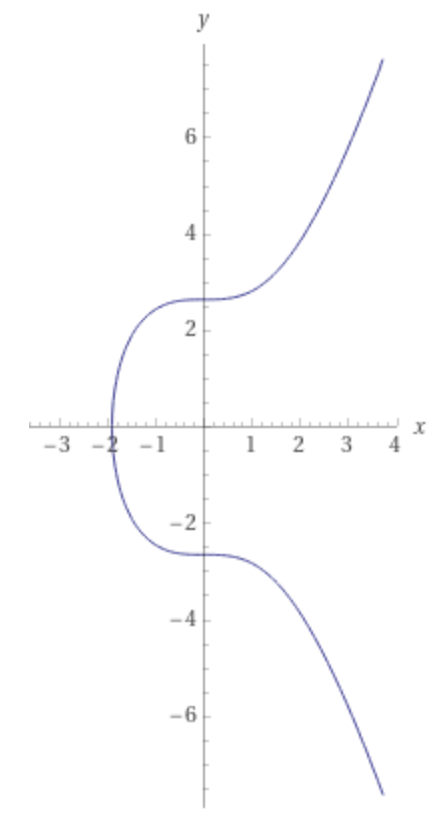
\includegraphics[width=.4\linewidth]{Pictures/bitcoinec.png}
  \caption{Figure 1:\ \(y^2 = x^3 +7\)}
  \label{fig:test1}
\end{minipage}%
\begin{minipage}{.5\textwidth}
  \centering
  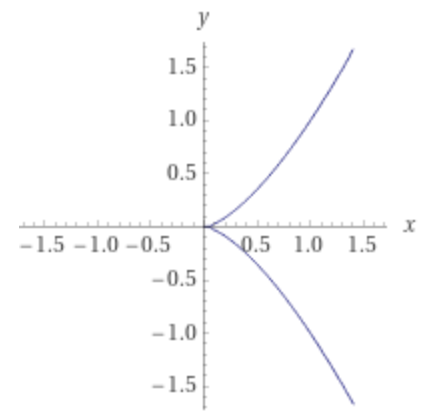
\includegraphics[width=.4\linewidth]{Pictures/y2x3.png}
  \caption{Figure 2:\ \(y^2 = x^3\)}
  \label{fig:test2}
\end{minipage}
\end{figure}

In general, elliptic curves are useful for zk-SNARKs because of the discrete logarithm problem, which is believed to be very hard to solve. Given a point \(g\) on the elliptic curve, and a multiple of that point, \(n*g\), it is impossible to solve n, even if \(g\) and \(n*g\) are given. In order to choose an elliptic curve that offers homomorphic hiding, we need to implement a mapping between our known numbers of the finite field \begin{math}\mathbb{F}_p\end{math} and a set of points on the elliptic curve (hidden space). Let \begin{math}\mathbb{F}_p\end{math} be a finite field of order p, whereby p is a large prime, e.g., if \(p=97\), then \begin{math}\mathbb{F}_p\end{math} \(=\{0, 1, 2, 3, ..., 96\}\) For this, we are going to take a generator point \(g = (x1,y1)\) that lies on the elliptic curve and multiply it with every element \({element}_i\) in \begin{math}\mathbb{F}_p\end{math}. For example, \(g + g = 2*g\) is calculated by putting a tangent line on \(g\), and wherever the line crosses the elliptic curve, we receive the result by using the opposite signs of that point. To arrive at \(2*g + g = 3*g\), the point \(2*g\) is used to draw a line to \(g\), see where the line further intersects with the elliptic curve, and use the opposite signs of that point to arrive at \(3*g\). This is repeated for every \(element\) in \begin{math}\mathbb{F}_p\end{math}. As a result, we have our finite field mapped to a hidden space on the elliptic curve. In summary, every \(element\) is hidden by
\begin{align}
    hh(element) = element * g
\end{align}
Additionally, we have to define what 0 and 1 are. The element 0 is the subtraction of a point on the elliptic curve, i.e., when point g goes to infinite. 1 is the point g itself.
Now, we have achieved homomorphic addition:
\begin{align}
    (A + B) \longrightarrow (A + B) * g = A*g + B*g
\end{align}

In order to use elliptic curve pairing to verify zk-SNARKs proofs, e.g., Groth16, we need to achieve a limited homomorphic multiplication operator. The hidden space is a group of points generated by the finite field elements and the generation point, \(g1\). Now, we want to choose a subgroup \(G1\) from that group. We choose that subgroup in a away that the number of elements we chose, \(r\), is a prime number too. Having found r, we can continue to choose the embedding degree of the elliptic curve. In Groth16, the proving key and verification key consist of G1 and G2 element, but we come to this later. The embedding degree \(k\) has to be found in a way that \(p^k-1|r\), i.e., is a multiple of. Let us use a minimal example to show how to arrive at \(G1, G2\).
Let us define an example base field \begin{math}\mathbb{F}_p\end{math} \(= \{0,1,2\}\) with \(p = 3\). We have found an embedding degree \(k=2\). In order to achieve our goal of creating a subgroup \(G2\), we need to extend our base field by a defining polynomial. This polynomial is of degree \(k\), and no element of our base field evaluates it to 0. In summary, we have:

\begin{align}
    \mathbb{F}_p = \{0,1,2\}, p = 3, k = 2
\end{align}

Defining polynomial for field extension \begin{math}\mathbb{F}_p^k\end{math}: 
\begin{align}
    f(x) = z^2 +1 \\
    f(0) = 1\\
    f(1) = 2\\
    f(2) = 5 mod 3 = 2
\end{align}

As shown in (17), none of the base field elements make f(x) evaluate to 0. In order to create the elements of the field extension \begin{math}\mathbb{F}_p^k\end{math}, we have to create all possible degree 2 polynomials out of the combinations of our base field \begin{math}\mathbb{F}_p\end{math}. For example, one possible polynomial with the coefficients from our base field is:

\begin{align}
    1*z^2+2*z+0 
\end{align}   
\begin{align*}
    (z^2+2*z)\mod (z^2+1) = 2*z-1\mod 3 = 2*z+2
\end{align*}
\(2*z+2\) is one element of the extension field \begin{math}\mathbb{F}_p^k\end{math}. In total, \begin{math}\mathbb{F}_p^k\end{math} has 9 elements, all calculated as in (21). In Summary, the elements of our extension field \begin{math}\mathbb{F}_p^k\end{math} are
\begin{align}
\{0, 1, 2, z, z+1, z+2, 2z, 2z+1, 2z+2\}
\end{align}

As shown in (22), the elements of the extension field are polynomials of degree up to \(k-1\). Addition and multiplication are defined in the way that coefficients are calculated \(\mod 3\) and polynomials \(\mod z^2+1\), the defining polynomial  
\(f(x)\) from (17).

Now, having our extension field, we can use it to create \begin{math}\mathbb{G}_2\end{math}, a subgroup of points of the same elliptic curve used for \begin{math}\mathbb{G}_1\end{math}, but with elements of \begin{math}\mathbb{F}_p^k\end{math}, instead of base field \begin{math}\mathbb{F}_p\end{math}. For this, we have to define points, whereby x and y coordinates are polynomials from \begin{math}\mathbb{F}_p^k\end{math}. \begin{math}\mathbb{G}_2\end{math} will consist of combinations from \begin{math}\mathbb{F}_p^k\end{math} in the form of \((x,y)\), which satisfy the elliptic curve. 

Pairings are bilinear maps that combine elements of two spaces to receive an element of a third space, e.g. matrix multiplication. In Groth16, the following pairing notation is used:

\begin{align}
    e: \mathbb{G}_1 \times \mathbb{G}_2 \to \mathbb{G}_T
\end{align}

The result of all steps performed previously is an incomplete homomorphic multiplication that enables us to check that the correct polynomial coefficients were used for \(A(x), B(x), C(x)\), as well as the same solution vector \(s\). It is incomplete, because not more than 2 elements can be multiplied. However, this just satisfies the use case for zk-SNARKS. 

\subsubsection{Groth16}

Now we covered all necessary basics to understand the Groth16 NIZK proof algorithm. In the following, we will cover the setup, proof and verification steps in Groth16.
Let us define the given parameters:\\

\begin{table}[ht]
    \centering
    \begin{tabular}{m{0.35\linewidth} | m{0.6\linewidth}}
        \centering
        \(n,m\) &  number of constraints, number of variables\\
        \hline \centering
        \begin{math}\mathbb{F}_p\end{math} & finite field of prime order p \\
        \hline \centering
         \begin{math}\mathbb{G}_1, \mathbb{G}_2, \mathbb{G}_T\end{math} & groups of points of prime order p satisfying an elliptic curve\\
         \hline \centering
         \begin{math}\mathbb{G}_1 \times \mathbb{G}_2 \to \mathbb{G}_T\end{math}& bilinear pairing \\
         \hline \centering
         \begin{math}g_T = e(g_1, g_2)\end{math}& generators with mapping \\
         \hline \centering
         \begin{math}\bigl\{A_i(X), B_i(X), C_i(X)\bigl\}_{i=0}^m\end{math} & encoded computation as result of R1CS and QAP three sets of polynomials of degree \(n-1\)\\
         \hline \centering
         \(Z(x) = (x-1)*(x-2)* \ (x-3)...(x-(n-1))\) &  minimal polynomial, known because n is known \\
         \hline \centering
         \(l\) & number of public inputs \\
         \hline \centering
         \((s_1,...,s_l)\) & elements of witness whose inputs are public (e.g., out = 35 in our example)\\
         \hline \centering
         \((s_{l+1},s_{l+2},...s_m)\) & elements of witness for secret input x, with \(s_0 = 1\) \\
    \end{tabular}
\end{table}

\subsubsection{Key generation}

The proving and verification key are obtained from the Common Reference String (CRS) via multi-party computation. From \begin{math}\mathbb{F}_p\end{math}, a set of random values is generated. This toxic waste (tw), or trapdoor, must be secret and forgotten from memory, because knowledge of it enables forged proofs. Note, that \begin{math}\tau\end{math} is the random point \(P\) from our examples. From the toxic waste, polynomial \(L_i(x)\) is defined:
\begin{align}
    tw = (\alpha, \beta, \gamma, \delta, \tau) 
\end{align}
\begin{align*}
    L_i(x) = \beta * A_i(X) + \alpha * B_i(X) + C_i(X)
\end{align*}
The CRS consist of \begin{math} \sigma = ([\sigma_1]_1,[\sigma_2]_2)\end{math}, which are elements of \begin{math} \mathbb{G}_1, \mathbb{G}_2\end{math}.

\begin{align}
    [\sigma_1]_1 = 
    &\ [(\alpha, \beta, \gamma, \delta, \\
    &\ 1, \tau, \tau^2, \tau^3, ..., \tau^{n-1}, \\
    &\ \frac{L_0(\tau)}{\gamma}, ..., \frac{L_l(\tau)}{\gamma}, \\
    &\ \frac{L_{l+1}(\tau)}{\delta}, ..., \frac{L_m(\tau)}{\delta})]_1 
\end{align}
\begin{align}
    [\sigma_2]_2 = [(\beta, \gamma, \delta, \ 1, \tau, \tau^2, \tau^3, ..., \tau^{n-1})]_2
\end{align}

\begin{itemize}
    \item (25): elements of the toxic waste
    \item (26): powers of \begin{math}\tau\end{math} of degree up to \(n-1\)
    \item (27): the polynomial is chosen from the set of polynomials of \(A(X), B(X), C(X)\), which corresponds to the place of the public input of the solution vector. In our starting example, \(out = 35\) is the public input (since this is our only public input, \(l=1\)). The public input is at third place in s. Hence, \(A_3(X), B_3(X), C_3(X)\) are chosen, evaluated at \begin{math}\tau\end{math} and multiplied by \begin{math} \alpha, \beta\end{math} according to (24).
    \item (28): Same as (27), but for the non-public inputs of s. All elements of \begin{math} [\sigma_1]_1 \end{math} are \begin{math}\mathbb{G}_1\end{math} elements, e.g., \begin{math}\alpha_1 = g_1 * \alpha\end{math}.
\end{itemize}

The proving key consists of the following elements:
\begin{itemize}
    \item \([(\alpha, \beta, 1, \tau, \tau^2, \tau^3, ..., \tau^{n-1}, \frac{L_{l+1}(\tau)}{\delta}, ..., \frac{L_m(\tau)}{\delta})]_1\)
    \item \([(1, \gamma, \delta)]_2\)
    \item circuit information about the polynomials:\\
    \(A_0(X), A_1(X), ..., A_m(X)\),\\
    \(B_0(X), B_1(X), ..., B_m(X)\),\\
    \(C_0(X), C_1(X), ..., C_m(X)\),\\
    \(Z(x) = (x-1)(x-2)(x-3)...(x-(n-1))\)\\
\end{itemize}

The verification key consists of the following elements:
\begin{itemize}
    \item \([(1, \frac{L_0(\tau)}{\gamma}, ..., \frac{L_l(\tau)}{\gamma})]_1\)
    \item \([(1, \gamma, \delta)]_2\)
    \item precomputed pairing \([\alpha * \beta]_T\), which is a \begin{math}\mathbb{G}_T\end{math} element
\end{itemize}

\subsubsection{Generating the proof}

Two random numbers \(r, t\) are generated from \begin{math}\mathbb{F}_p\end{math}, that are used to compute

\begin{enumerate}
    \item \begin{math} A= \alpha + s_0*A_0(\tau) + s_1*A_1(\tau) + ... + s_m*A_m(\tau) + r\delta\end{math}
    \item \begin{math} B= \beta + s_0*B_0(\tau) + s_1*B_1(\tau) + ... + s_m*B_m(\tau) + t\delta\end{math}
    \item \begin{math} C= \frac{s_{l+1}L_{l+1}(\tau)}{\delta} + \frac{s_{l+2}L_{l+2}(\tau)} + ... +\frac{s_{lm}L_{lm}(\tau)}{\delta} + \frac{H(\tau)Z(\tau)}{\delta} + At + Br - rt\delta\end{math}
\end{enumerate}

The proof \begin{math}\pi\end{math} consists of two elements from \begin{math}\mathbb{G}_1\end{math} and one element from \begin{math}\mathbb{G}_2\end{math}:
\begin{align}
    \pi = ([A]_1, [B]_2, [C]_1)
\end{align}

\subsubsection{Verification}

In Groth16, three pairings are checked during verification. \begin{math}[\alpha * \beta]_T\end{math} is a precomputed pairing and is made available in the setup phase. The verification computation receives proof \begin{math} \pi\end{math} and accepts it only if the following equation holds:
\begin{align}
    [A]_1 * [B]_2 = [\alpha]_1[\beta]_2 + \bigl[\frac{s_0L_0(\tau)}{\gamma}+ \frac{s_1L_1(\tau)}{\gamma} + ... + \frac{s_lL_l(\tau)}{\gamma}\bigr]_1 * [\gamma]_2 + [C]_1 * [\delta]_2
\end{align}

As shown in (31), the following three pairings are needed to be checked:

\begin{itemize}
    \item \(e([A]_1, [B]_2)\)
    \item \begin{math}
        e(\bigl[\frac{s_0L_0(\tau)}{\gamma}+ \frac{s_1L_1(\tau)}{\gamma} + ... + \frac{s_lL_l(\tau)}{\gamma}\bigr]_1 , [\gamma]_2)
    \end{math}
    \item \begin{math}
        e([C]_1, [\delta]_2)
    \end{math}
\end{itemize}

Let us evaluate the verification equation in (31). The left hand side evaluates as follows:

\begin{equation*}
\begin{split}
    [A]_1 * [B]_2 = [A*B]_T &= [\alpha + s_0*A_0(\tau) + s_1*A_1(\tau) + ... + s_m*A_m(\tau) + r\delta]_1 \ *\\
    &\ \ \ \ [\beta + s_0*B_0(\tau) + s_1*B_1(\tau) + ... + s_m*B_m(\tau) + t\delta]_2 \\
    &= [(\alpha + A(\tau) + r\delta) * (\beta + B(\tau) + t\delta)]_T\\
    &= [\alpha * \beta]_T + [\alpha * B(\tau)]_T + [\alpha * t\delta]_T \ + [A(\tau) * \beta]_T \ + \\
    &\ \ \ \ [A(\tau) * B(\tau)]_T + [A(\tau) * t\delta]_T + [r\delta * \beta]_T + [r\delta * B(\tau)]_T +\\
    &\ \ \ \ [r\delta * t\delta]_T \\
    \\
    &= [A(\tau) * B(\tau)]_T \textcolor{blue}{\ +\ [\alpha * \beta]_T + [\alpha * B(\tau)]_T + [\alpha * t\delta]_T} \\
    &\ \ \textcolor{blue}{+ [A(\tau) * \beta]_T \ + [A(\tau) * t\delta]_T + [r\delta * \beta]_T + [r\delta * B(\tau)]_T} \\
    &\ \ \textcolor{blue}{+ [r\delta * t\delta]_T}
\end{split}
\end{equation*}

The right hand side evaluates to:
 \begin{equation*}
     \begin{split}
    &=[\alpha]_1[\beta]_2 + \bigl[\frac{s_0L_0(\tau)}{\gamma}+ \frac{s_1L_1(\tau)}{\gamma} + ... + \frac{s_lL_l(\tau)}{\gamma}\bigr]_1 * [\gamma]_2 + [C]_1 * [\delta]_2 \\
    &=[\alpha * \beta]_T + [(s_0L_0(\tau) + s_1L_1(\tau) + ... + s_lL_l(\tau))]_T + [(s_{l+1}L_{l+1}(\tau) + s_{l+2}L_{l+2}(\tau) + ... \\
    &\ \ \ + s_{lm}L_{lm}(\tau)) + H(\tau)Z(\tau) + At\delta + Br\delta - rt\delta\delta]_T
     \end{split}
 \end{equation*}

Now, we can replace A and B. We also see that the middle of the equation is \(L_i(\tau)\).
 \begin{equation*}
     \begin{split}
     &=[H(\tau) * Z(\tau) + C(\tau)]_T \textcolor{blue}{\ +\  [\alpha * \beta]_T + [\alpha * B(\tau)]_T + [\alpha * t\delta]_T + [A(\tau) * \beta]_T} \\
     &\ \ \ \textcolor{blue}{+ [A(\tau) * t\delta]_T + [r\delta * \beta]_T + [r\delta * B(\tau)]_T + [r\delta * t\delta]_T}
     \end{split}
 \end{equation*}

Eventually, we get the equality check we wanted to achieve (13). The use of the secret encoded values \(\alpha, \beta\) of the toxic waste (24) force the prover algorithm to use the same coefficients of the solution vector (witness) to compute \(A(X), B(X), C(X)\). \(\gamma, \delta\) ensure that the public inputs of order \(l\) are independent from the solution vector (witness). In order to achieve the zero-knowledge aspect, \(r, s\) are used to randomly shift the proof.
    


    
\begin{comment}
-table with extension field elements and x^3 and y^2, then explaining how to get there and how to pick points satisfying the elliptic curve in example
- then new sub chapter on bilinear mapping g1 x g2 -> gt, we have achieved limited homomorphic multiplication for zkSNARKs
- we need to calculate B in G2 for the pairing, but also in G1 in order to get C
\end{comment}

\section{Plonk-based zk-DApp}
- definition of plonk and comparison to groth16/differences and why
\subsection{Summary of Requirements}
- use case support system for predictive maintenance
\subsection{Implementation and Results}
- description of circom, snarkjs implementation
- graphic of how the zkDApp works
\subsection{Evaluation}
- comparison of groth16 and plonk performance
- limitations of the implementation
- future outlook with turboplonk

\section{Verification Mechanism Architecture}
-create a architecture for verification mechanisms in Rapado, based on Sedlmeier, Völter, Strüker (2021):
-->proof membership in a merkle tree? data structure of parts, certificates

- Campanelli et al 2022: improvement on zkSNARKS with Merkle Trees -->HARISA, could be used for the architecture

- build zk DAPP for document verification with circom snarkjs on hardhat test network
- maybe use snarkjs Groth16 first and then PLONK as future outlook, when TurboPLONK support will come in snarkjs
